% ************ Chapter 5 ************
\chapter{Desenvolvimento e implementação} 
\label{cap:5}


\section{Desenvolvimento da primeira fase do projeto}
A primeira fase do projeto foi desenvolvida entre as semanas 4 e 6. Este desenvolvimento consistiu criar os modelos (models), desenhar cada um dos ecrãs das aplicação (views) e os controladores (controllers) dos casos de uso Marcar Ponto, Registo de Recolha, Registo de Produção, Registo de Produto Acabado e Registo de Saída de Produto Acabado.\\
Utilizando os recursos do próprio Laravel, os models foram gerados automaticamente com base na estrutura da base de dados, atraves do recurso de migrations. As migrations são um ficheiros que descrevem a estrutura de uma tabela da base de dados. Servem para poder criar ou alterar tabelas na base de dados sem que o programador tenha de se preocupar com o DBMS\label{sym:DBMG}.\\
O Laravel inclui o Artisian, uma interface de linha de comandos que disponibiliza uma um conjunto de uteis para a construção da aplicação\cite{Laravel}.
Para criar uma migration e o seu respetivo model basta executar no terminal o seguinte comando

\begin{lstlisting}
$ php artisian make:migration NomeDaMigration -m
\end{lstlisting}

\noindent
E serão gerados os ficheiros de migration e model. Após inserir a estrutura que se pretende para as tabelas da base de dados e suas relações nos ficheiros de migrations, usando o comando

\begin{lstlisting}
$ php artisian migrate
\end{lstlisting}

\noindent
As tabelas da base de dados seriam criadas exatamente da forma como foram descritas.\\
Finalizada a criação dos models, iniciou-se o processo de desenho de cada uma das views. Nesta fase já se sabia que muitos elementos se iriam repetir ao longo da interface, uma consequência direta da coesão da interface. Por esse motivo procurou-se desde cedo isolar alguns elementos de cada um dos ecrãs, como descrito na figura \ref{fig:ui_fabrica_camadas}, para que evitar reescrever código, além de simplificar futuro trabalho de manutenção. Definiu-se então que todas as páginas seriam construídas em cima de uma mesma base. Dependendo da página solicitada era incluída a view a ela referente. No caso dos formulários era ainda incluídos os botões de ação (Guardar, Limpar e Cancelar), com a excepção do formulário de Registo de Ponto. Por fim, os elementos de dropdown de seleção de Colaborador e Ponto de Recolha eram ainda incluídos de outros dois ficheiros independentes. 
\begin{figure}[htbp] 
	\begin{center}
		% Requires \usepackage{graphicx}
		\includegraphics[width=\textwidth,keepaspectratio]{figuras/camadas_fabrica.png}
		\caption{Camadas da página Aplicação Fábrica}
		\label{fig:ui_fabrica_camadas} 
	\end{center}
\end{figure}

\noindent
Estas inclusões de ficheiros foram produzidas através do recurso Blade fo Laravel. O Blade é um mecanismos de modelagem incluso no Laravel que ao contrario da maioria dos mecanismos de modelagem premite o uso de código PHP na própria view. São ficheiros com a extensão .blade.php e estão, normalmente, dentro do diretório resources/views\cite{Laravel}.

\subsection{Implementação da primeira fase}
Conforme os requisitos do projeto, a primeira fase so poderia ser implementada após as funcionalidades da aplicação existente na fabrica (Registo de ponto, de recolhas, de produção, de produto acabado e de saída de produto acabado). Só após estas funcionalidades bem testadas e a coesão do novo sistema se poderia implementar o novo sistema. No final da sexta a administração concordou que o sistema já tinha condições para ser implementado, mas como a semana seguinte coincidia com a ultima semana do mês de maio a administração solicitou que a implementação fosse adiada uma semana visto que não teria tempo de adaptar todas as ferramentas de analises de dados a tempo de fazer a produção dos relatórios mensais. Ficou então decidido que a implementação iria ocorrer na semana 8 e durante a semana 7 iria continuar o desenvolvimento do sistema além de continuar os testes à versão a ser implementada. De forma a manter a versão estavél nessa condição criou-se no repositório uma segunda branch chamada "release".

\subsection{Configuração do servidor e migração de dados}
A implementação do projeto teria de ocorrer durante o fim de semana pela necessidade de não haver registos durante o processo de implementação e migração, ou seja, teria de ser enquanto a fábrica está parada.\\
No dia da implementação o servidor já estava montado e sistema operativo instalado, restando apenas instalar o servidor web, interpretador php, sistema de gestão de base de dados, fazer a migração da base de dados e instalar o sistema de informação. Após a instalação dos softwares necessários passou-se para a migração da base de dados. A migração da base de dados consistiu na importação do ficheiro .accdb (Microsoft Access) para a base de dados nova. Concluída a importação, foi feito um conjunto de querys de inserção da informação que constava na base de dados antiga. Este não foi um processo sempre linear, nomeadamente nas tabelas que foram divididas porque involveu querys mais complexas com joins.
No final da migração foram efetuados vários querys para comparar a informação nas duas bases de dados.\\
O supervisor da empresa, o Engº Telmo Azevedo, decidiu tomar este momento como um momento didático, optando por construir as querys à frente do estudante para assim poder passar alguns conhecimentos de sobre SQL, no lugar de simplesmente preparar as querys com antecedência e simplesmente as executar no momento da migração, uma vez que a migração da base de dados não fazia parte dos requisitos do projeto.\\
Finalizada a migração da base de dados, ocorreu a instalação do sistema de informação. para este processo bastou clonar a branch release do repositório uma vez que todo o desenvolvimento foi pensado para no momento da implementação as configurações do sistema informação serem as mesmas tanto no computador de desenvolvimento quanto no servidor de produção.\\
Ocorrem alguns problemas no pós instalção pois a aplicação não estava a conseguir comunicar com a base dados, problema que foi resolvido através de uma configuração na firewall do servidor, que por padrão bloqueava todos os pedidos de entrada no servidor.\\
Para concluir o processo criou-se um utilizador destinado aos administradores, para que estes pudessem aceder ao Painel e criou-se atalhos no ambiente de trabalho de todos os computadores da empresa para ter um acesso fácil à aplicação. Após executar o atalho criado uma nova janela do browser era aberta, aparecendo o menu da aplicação de fábrica (figura \ref{fig:posinstall_fabrica_menu}.) 
\begin{figure}[htbp] 
	\begin{center}
		% Requires \usepackage{graphicx}
		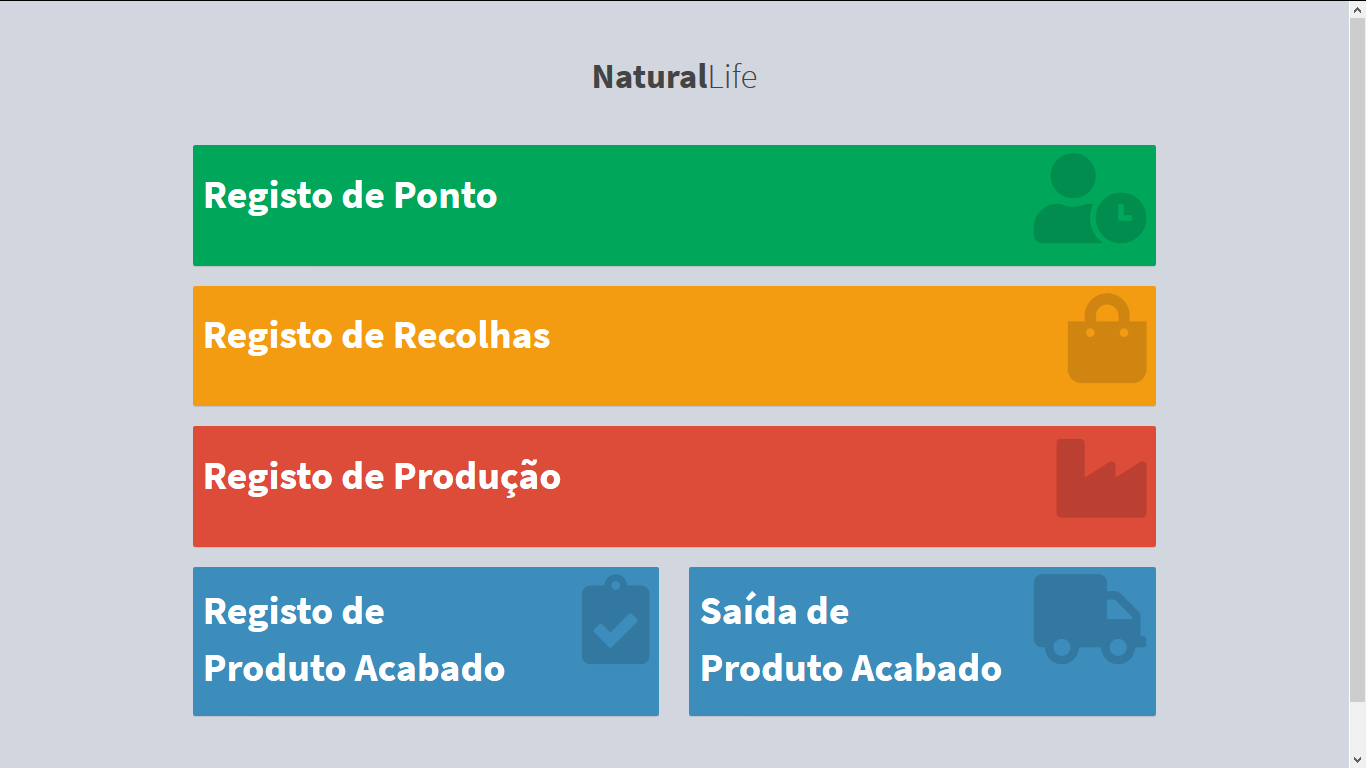
\includegraphics[width=0.90\textwidth,keepaspectratio]{figuras/AppPhp/0-menu_1_fase.png}
		\caption{Menú da Aplicação Fábrica na primeira fase}
		\label{fig:posinstall_fabrica_menu} 
	\end{center}
\end{figure}
\subsection{Primeiro dia de utilização}
O primeiro dia utilização foi a segunda-feira da semana oito, dia 3 de junho de 2019. Não decorreu nenhum problema durante todo o dia, tendo sido apenas apontados detalhes de user experience, por exemplo os colaboradores esperavam poder usar a virgula para separar as casas decimais no lugar do ponto. Apesar de não ser um requisito do sistema usar a virgula como separador das casas decimais essas modificações foram implementadas pois o trabalho necessário para as fazer era minimo se comparado com a melhoria da user experience dos colaboradores.

\subsection{Segunda fase de implementação}
Durante a segunda fase de implementação, as funcionalidades passaram a ser disponibilizadas após concluir o processo de teste. Este processo não era um processo tão rigoroso como o da primeira fase, mas também não se fazia necessário porque deixou de existir a possibilidade da fábrica ser obrigada a parar por algum erro nas funcionalidades básicas da aplicação. No entanto as funcionalidades so passavam a estar disponíveis na versão em produção após o aval do supervisor. Foi nesta fase que alem de se desenvolver toda a aplicação Painel, foram implementadas as funcionalidades 2ª via de código de barras e Completar recolha.

\section{Feedback obtido}
Durante os testes feitos pela administração antes da primeira execução, o feedback obtido foi positivo e no momento que a administração decidiu experimentar o sistema com alguns colaboradores, a reação foi similar. Os primeiros comentários feitos referiram-se à simplicidade e facilidade da interface apresentada. Referiram ainda que as mensagens de erro eram muito mais preceitivos que as anteriores.
Estes comentários mantiveram-se ao longo de todo o período de desenvolvimento da plataforma, demonstrando assim que o sistema desenvolvido foi de encontro com as expectativas dos seus utilizadores.

\section{Execução do projeto} 
Como forma de avaliar o desenvolvimento do projeto, foi construído um gráfico (figura \ref{fig:burndown_chart}), denominado \textit{burndown char}, que demonstra a relação entre os objetivos a cumprir com o período do projeto. A linha de cor azul refere-se ao que era exptavél que acontecesse, um desenvolvimento constante no qual o projeto é entregue no último dia do período, com todos os objetivos concluídos. A laranja é possível observar a evolução real do trabalho. Desta linha é relevante analisar que durante as primeiras três semana a evolução do projeto ficou à quem do esperado, devido ao processo de estudo da empresa e das ferramentas a serem utilizadas. Finalizado esse processo a linha de execução superou a previsão culminando com a conclusão do projeto uma semana antes do previsto.
\begin{figure}[htbp] 
	\begin{center}
		% Requires \usepackage{graphicx}
		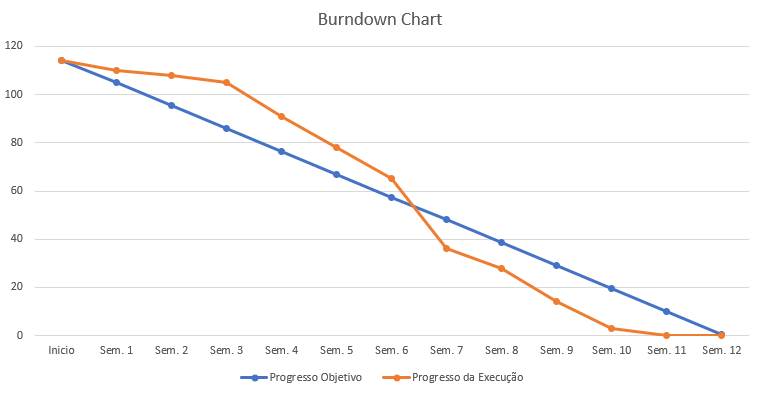
\includegraphics[width=0.90\textwidth,keepaspectratio]{figuras/burndown_chart.png}
		\caption{\textit{burndown char} da excussão do projeto}
		\label{fig:burndown_chart} 
	\end{center}
\end{figure}